\chapter{Conclusion}

In this dissertation, the quantum machine learning algorithms QkNN and QSVM were explored along with Grover's quantum based search algorithm and various data encoding techniques. The runtime advantages claimed for quantum systems were also evaluated.


We achieved the goal of implementing theoretical research and the theoretically based implementations of these algorithms and data encoding techniques. This work delivered them in a modular manner depicting the advantage not just of various quantum cloud computing providers but also the algorithms chosen and the encoding techniques available.


 While building on the work of \citep{sharmaQeml}, the number of tested dimensions was increased from 10 to 100, 150 and 500. With these increases, the run-time advantages claimed for QkNN and some variations of QSVM were observed in benchmarking.
 
 
While the implementation of the JKU classical quantum simulation was initiated, there is still more work to be done in order to see this implementation to completion. However, the main objective of providing an accessible and centralised pathway into quantum and quantum enhanced programming was achieved through the presentation of concise introductory information
%in the background section 
and the implementation of various modular components in an illustrative and accessible manner.

\section{Further Studies}
Looking ahead, the fields of quantum computing and quantum machine learning continue to innovate. While carrying out this dissertation we saw the release of a new quantum cloud system by Baidu Research called Paddle Quantum \citep{Baiduo}. Paddle Quantum is a quantum machine learning development toolkit that can help scientists and developers quickly build and train quantum neural network models and provide advanced quantum computing applications. Another example of continuing innovation is a new approach to quantum error correction from AWS Center for Quantum Computing that would encode the information into a protected qubit using many other physical qubits \citep{Amaz}. As quantum computers are quite susceptible to noisy hardware and different types of errors and interference -- as we discussed in Section \ref{NoiseErrInter} -- this possible advancement could enable quantum computers to be able to \emph{execute quantum algorithms despite the “noisy hardware” that remains prone to errors} \citep{Amaz}. This in turn could see our accuracy results improve significantly.

\subsection{Modular Tool Improvements}
In the scope of a modular tool, there is still more work to be done. To begin with, the addition of current quantum machine learning algorithms would expand on the modular tool's capabilities. Algorithms such as Quantum k-Means by \citeauthor{Khan2019} \citep{Khan2019}, for further grouping of new data points, would be generally useful in a modular system. Currently, to use this modular tool, one has to have the full code present and run all of it, calling the required  modular components into the final circuit. It would be desirable to streamline this approach. One such implementation would see the tool being encapsulated in a library. This would allow one to call the desired modular components using the library's API calls without having the full code present. %Thus, providing a more central black box that one could build upon. 

As this work was coming to a close, IBM's 15 qubit quantum machine became unavailable for public use. The current largest publicly available IBM quantum computer allows for a circuit with a maximum depth of five. This change in circuit depth may not affect the current QSVM implementation as it is a hybrid implementation with only quantum encoded kernel data. The QkNN circuit implemented in this dissertation has a circuit depth of nine qubits and so, at the time of writing, can no longer be run on publicly available IBM quantum computers. %Some 
Compression techniques, such as a reduction in the number of additions, could be implemented to reduce the number of qubits used. If %the current maximum 
IBM's quantum computer continues to only allow circuits with a maximum depth of five, %it could explored
a further exploration into the effect that %the type of 
compression could have on the QkNN circuit's ability to perform adequate classification could be undertaken.

%just as the work was coming to a close and ....it could effect the QkNN with the larger circuit depth, but with compression of the QkNN but it might affect its ability to implement, but with QSVM might be a problem


\subsection{ Applications of Grover's Algorithm: \citeauthor{MarkSwee}}

During our discussion on Grover's Search algorithm in Section \ref{GrovImp}, we touched on its ability to have repetitions by increasing of the count size during re-measurement. 


%%%%%%%%%%%%%%%%%%%%%%%%%%%%%%%%%%%%%%%%
\begin{figure}[h!]
      \centering
      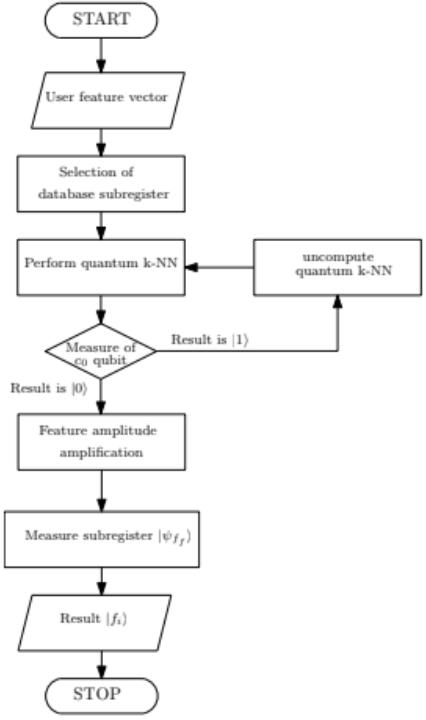
\includegraphics[scale=0.5]{background/RCC.png}
      \caption{Control flow of proposed quantum recommendation system
      \citep{MarkSwee}}
      \label{QRec}
\end{figure}
%%%%%%%%%%%%%%%%%%%%%%%%%%%%%%%%%%%%%%%%

In the quantum recommendation system in Figure \ref{QRec}, the use of repetition would enable this system to be  implemented. The addition of a \emph{feature amplitude amplification} component would further allow for a quantum recommendation system to be viable, thus producing new analytical comparisons against the classical recommendation system application. More details of this solution are discussed in \emph{Recommendation systems with the quantum k-NN and Grover algorithms for data processing} by % M.Sawerwain and M.Wróblewski 
 \citeauthor{MarkSwee}.

Continuing with Grover's Search, as it is a quantum based algorithm -- not derived from a classical algorithm -- there is no exact classical version we could compare it to. However, \citep{GroverCompared} compared Grover's Search algorithm to other classical search algorithms, namely Binary and Linear search. The paper found that Grover's Search algorithm did not outperform other search algorithms. However, the researcher executed Grover's search using a quantum simulator and not a real quantum device. Looking ahead, this research could be re-evaluated  using the quantum machines that are currently available, in order to really compare Grover's quantum advantage to classical search.

\subsection{JKU Simulator}
As previously stated, the JKU simulator allows for quantum algorithms to be executed in a classical environment. It has been developed as an open source tool that is, unfortunately, currently producing errors. Further research and development into this or other similar systems is necessary. This would not only allow a circuit to keep its existing quantum advantages, but it would also facilitate a more comparative analysis between classical machine learning algorithms, their quantum parts and also quantum centered algorithms such as Grover’s Search. 

\subsection{Quantum Noise and Interference}

Quantum noise and interference increases in proportion to circuit depth. There exist current error correction implementations that require multiple execution repetitions. While these techniques reduce some noise and errors, they are only applicable to smaller circuit designs. Another approach would involve increasing the current maximum number of qubits available in a quantum system. For example, if we wished to run Shor’s algorithm \citep{shor_lowB} well enough to factor, say, a number 1,000 bits long -- roughly the size used in some internet encryption schemes -- the system will need to maintain logical qubits with a part-in-1-billion error rate \citep{cho_2020}. That may require entangling a grid of 1,000 physical qubits to safeguard a single logical qubit. By current research, this is a prospect that will take generations of bigger and better quantum computing chips \citep{ADCho}. Quantum error correction and noise mitigation are critical issues, solutions to which would help propel quantum computing into the commercial arena \citep{Amaz}% out of its current majority based research space, in hopes to become commercially viable.

It is still early days for quantum algorithms as they do not provide the same or a higher level of accuracy as classical methods. This, coupled with the resource-intensive and time-consuming nature of quantum computing queues \footnote{While quantum computers execution times are reasonably fast, the queuing time to use a quantum machine can be more than three hours. The wait time depends on the number of active jobs waiting to be executed.}, means that quantum machine learning algorithms are not yet suitable for general commercial use. 
As quantum computing and quantum machine learning continues to improve, it is hoped that these obstacles will diminish over time. We could see strides made to increase the scale of quantum computers to reduce resource load, noise reduction for greater consistency and an uptick in the open source community permitting 
more accessible and centralised theoretical knowledge, implementation know-how and high quality documentation. 

As quantum machines grow in size and become more accessible, we can continue to build on work such as is presented in this dissertation and the research of others with the current technology at hand.
